\documentclass[11pt, a4paper]{article}

%===============================================================================
% PACKAGES
%===============================================================================
\usepackage[utf8]{inputenc}
\usepackage[T1]{fontenc}
\usepackage{amsmath}              % For mathematical formulas
\usepackage[margin=0.8in]{geometry} % For setting page margins
\usepackage{graphicx}             % To include graphics
\usepackage{hyperref}             % For clickable links
\usepackage{xcolor}               % For colors
\usepackage{amssymb}              % For symbols like arrows
\usepackage{fancyvrb}             % For the pseudocode box
\usepackage{float}                % For improved figure placement control

%===============================================================================
% DOCUMENT & HYPERLINK SETUP
%===============================================================================
\hypersetup{
    colorlinks=true,
    linkcolor=blue,
    filecolor=magenta,      
    urlcolor=blue,
}

%===============================================================================
% TITLE
%===============================================================================
\title{\textbf{Teaching an Agent to Navigate a Risky World: \\ A Q-Learning Adventure}}
\author{\Large\textbf{Team 01}  \\Jeevan Hebbal Manjunath, Varun Karthik, Yeshwanth Reddy Gurreddy}
\date{\today}

%===============================================================================
% DOCUMENT START
%===============================================================================
\begin{document}

\maketitle

\begin{abstract}
In this report, we explore how a simple agent can learn complex, intelligent behavior through pure trial and error. We apply the Q-learning algorithm to a classic gridworld problem, a world filled with rewards, penalties, and unpredictable movement. Through a comprehensive analysis of the agent's learning process, hyperparameter tuning, and final strategies in both standard and high-risk environments, we demonstrate its remarkable ability to adapt its behavior in response to potential danger.
\end{abstract}

\hrule
\vspace{1em}

%===============================================================================
\section{The Challenge: A Risky Gridworld}
%===============================================================================
Imagine a robot trying to find its way through a maze. The floor is slippery, so moving forward might cause it to slide sideways. The maze has a goal with a prize, but also a dangerous trap. This is exactly the challenge we've set for our learning agent.

The world is a $3 \times 4$ grid. The agent's mission is to get from the start at (1,1) to the prize at (4,3), which gives a `+1` reward. To make things harder, there's a wall at (2,2), a living penalty of `-0.04` for every move, and the agent's movement is stochastic—it only follows its intended direction 80\% of the time.

%===============================================================================
\section{Our Approach: Learning from Experience}
%===============================================================================
How can an agent learn with no initial instructions? We used Q-learning, a powerful reinforcement learning technique.

\subsection{The ``Cheat Sheet'' Analogy}
At its heart, Q-learning is like creating a ``cheat sheet'' (called a \textbf{Q-table}) for the agent. This cheat sheet has a score for every possible action in every possible square. A high score says ``This is a great move!'' while a low score says ``Avoid this!''

Initially, the agent knows nothing, so all the scores are zero. But as it explores the world, it constantly updates the cheat sheet based on the rewards and penalties it finds. The formula it uses to update the scores is:

\begin{equation}
Q(s, a) \leftarrow Q(s, a) + \alpha [r + \gamma \max_{a'} Q(s', a') - Q(s, a)]
\end{equation}

This looks complex, but it simply means: ``The new score for this move is a blend of the old score and any new information we just learned.''

\subsection{The Learning Algorithm}
The agent's training process is a continuous loop of exploring and updating its cheat sheet. To make sure it doesn't just stick to the first path it finds, we use an $\epsilon$-greedy strategy: most of the time it follows its cheat sheet, but sometimes it tries a random move, just to see what happens. This randomness (exploration) fades over time as the agent becomes more confident.

\begin{center}
\begin{BVerbatim}[frame=single, label=Algorithm Pseudocode]
Initialize the Q-table with all zeros for every state-action pair.
Set the learning parameters (alpha, gamma, epsilon).

For a large number of episodes:
    1. Place the agent at the START state.

    2. While the agent has not reached a terminal state (prize or trap):
        a. Decide whether to explore or exploit:
           --- With probability epsilon, choose a random action.
           --- Otherwise, choose the best action from the Q-table for the current state.

        b. Perform the chosen action.
        
        c. Observe the reward and the new state.
        
        d. Update the Q-table score for the action just taken using the Q-learning formula.
        
        e. Move to the new state.

    3. Slightly decrease epsilon to encourage less exploration over time.
\end{BVerbatim}
\end{center}

%===============================================================================
\section{Discussion of Findings}
%===============================================================================
The Q-learning agent successfully learned to navigate the gridworld. Analyzing its learning process and final strategies reveals key insights into how the algorithm operates and adapts.

\subsection{The Crucial Role of Hyperparameters}
The agent's learning effectiveness is highly dependent on tuning its core hyperparameters ($\alpha, \gamma, \epsilon$). Figure~\ref{fig:hyperparameter_summary} provides a high-level conceptual overview of their effects.

\begin{itemize}
    \item \textbf{Learning Rate ($\alpha$):} Controls how \textbf{impressionable} the agent is. A high $\alpha$ leads to faster learning but can be unstable, while a low $\alpha$ is stable but slow.
    
    \item \textbf{Discount Factor ($\gamma$):} Controls how \textbf{farsighted} the agent is. A high $\gamma$ is essential for prioritizing long-term rewards like the `+1` prize over short-term penalties.
    
    \item \textbf{Exploration Schedule ($\epsilon$ decay):} A \textbf{decaying schedule} is best. The agent starts with high randomness to explore, then gradually reduces it to exploit the optimal path it has found.
\end{itemize}

\begin{figure}[H]
    \centering
    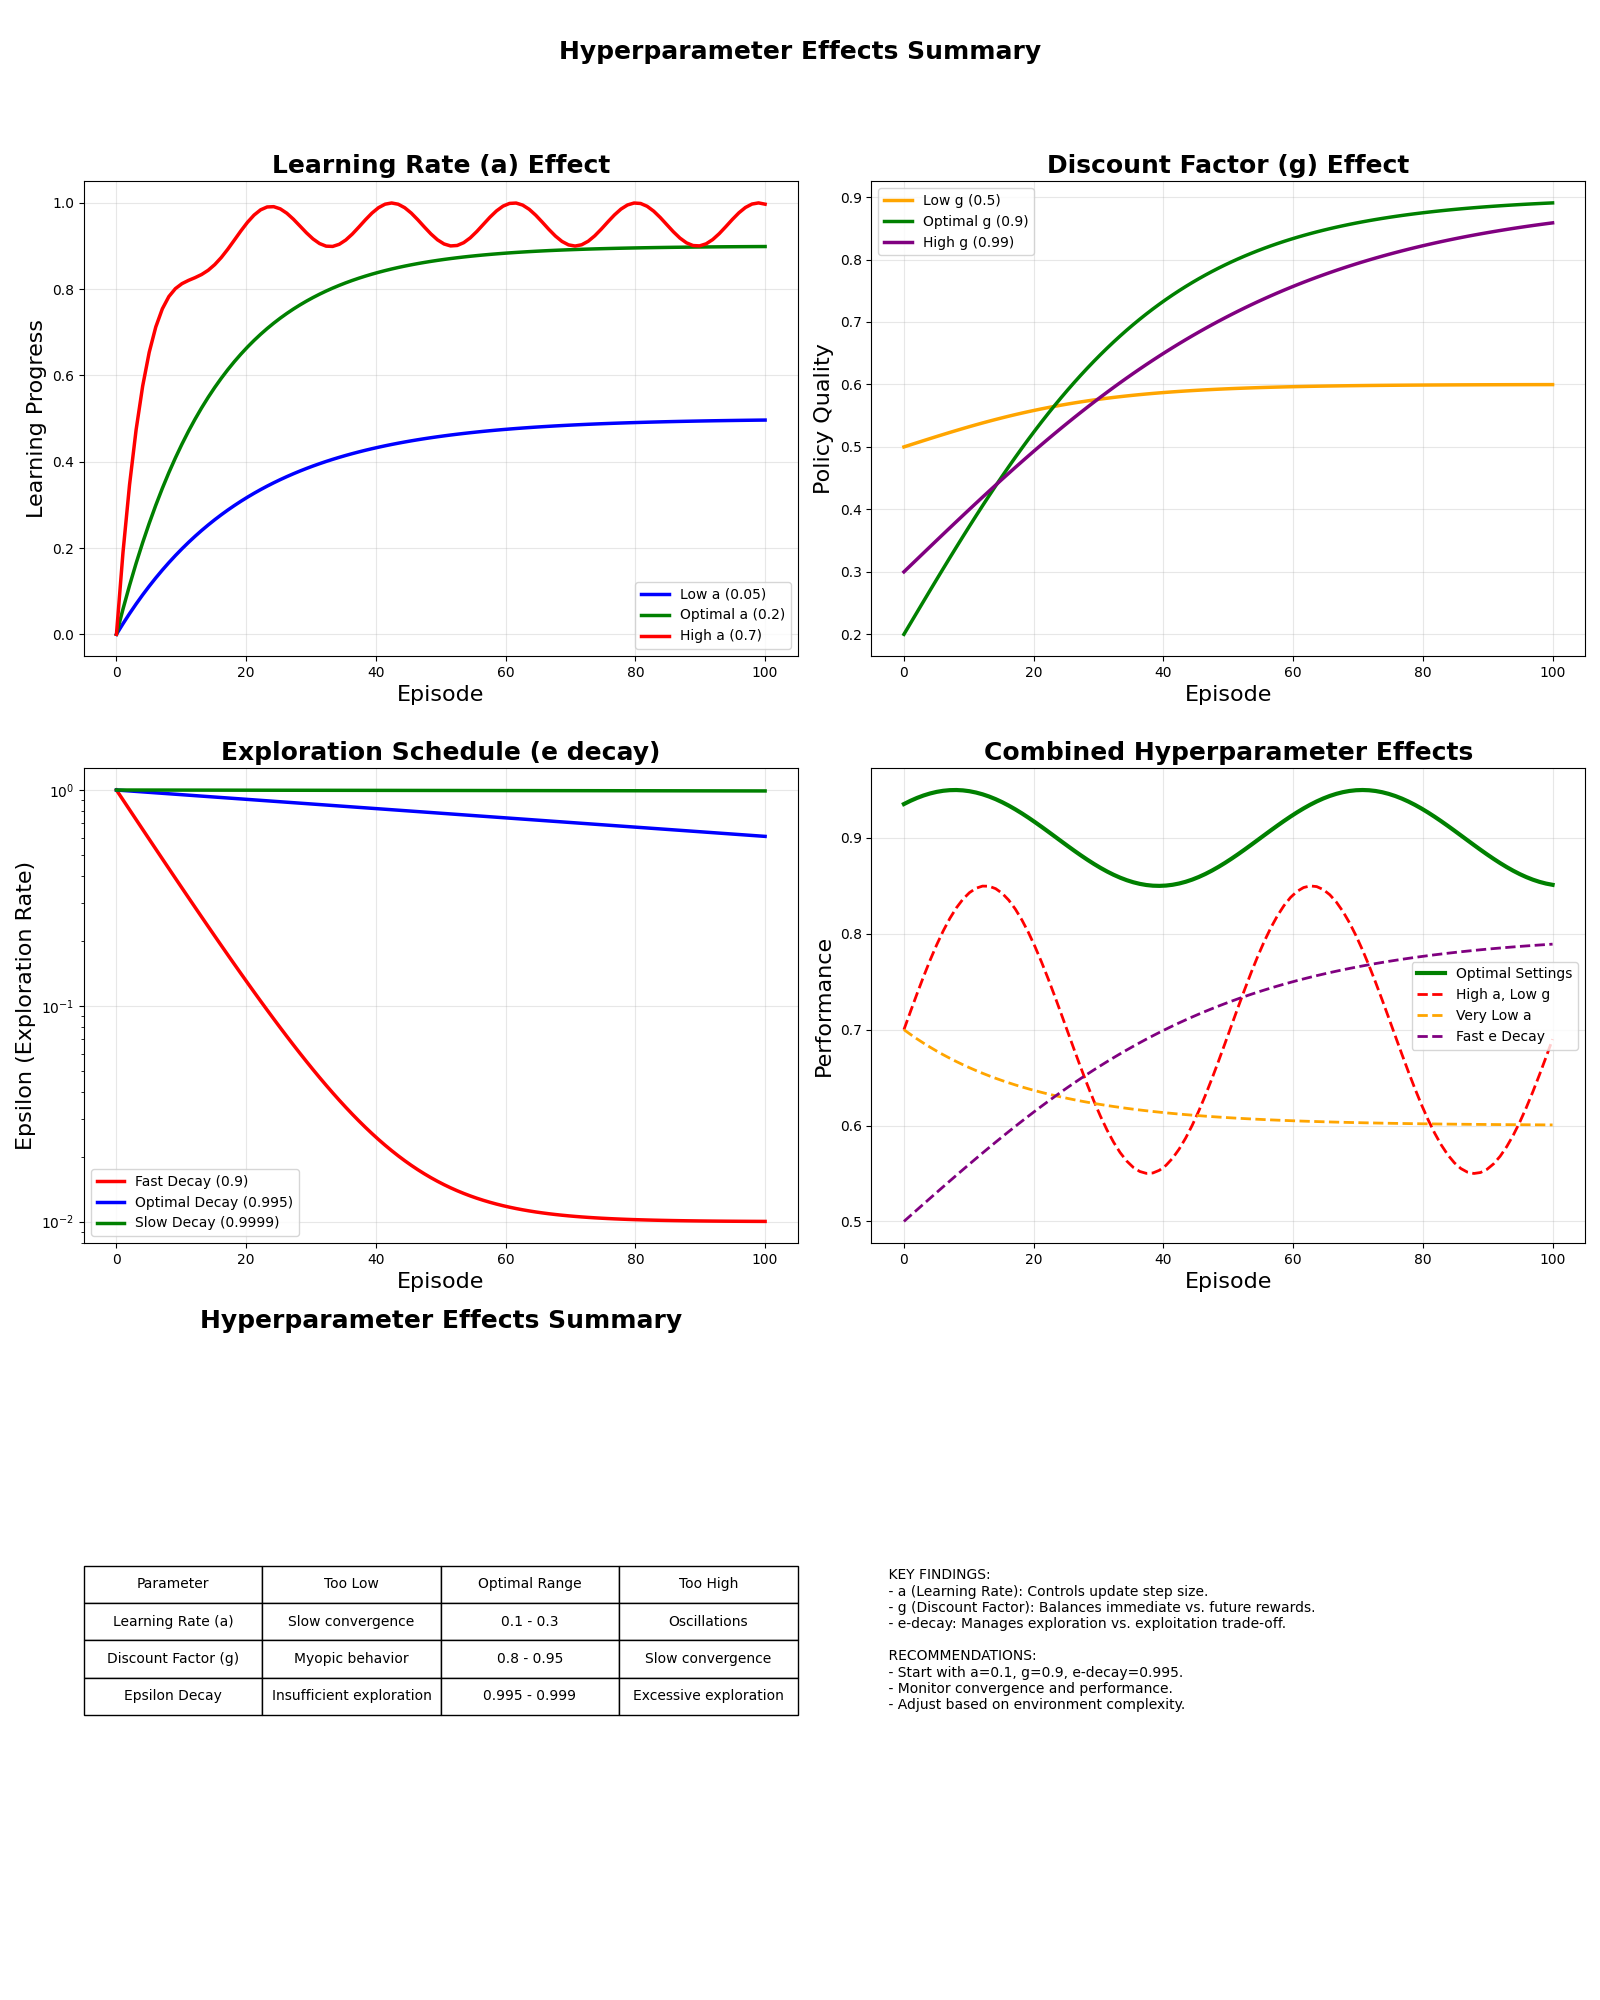
\includegraphics[width=0.9\textwidth]{images/hyperparameter_effects_summary.png}
    \caption{Conceptual overview of hyperparameter effects on Q-learning performance. Learning rate ($\alpha$) controls update speed, discount factor ($\gamma$) determines farsightedness, and $\epsilon$ decay balances exploration vs exploitation.}\label{fig:hyperparameter_summary}
\end{figure}

A more detailed, data-driven analysis is presented in the following figures. This comprehensive plot reveals several key trade-offs:
\begin{itemize}
    \item Figure~\ref{fig:hyperparameter_alpha} demonstrates the critical balance between learning speed 
    and stability in the learning rate parameter. Low values ($\alpha < 0.1$) lead to slow, overly 
    conservative learning that may not converge within reasonable time frames. High values 
    ($\alpha > 0.5$) cause erratic, unstable performance where new experiences override 
    previous learning too aggressively. The optimal range ($\alpha \approx 0.1-0.3$) achieves 
    rapid initial learning followed by stable convergence.
    \item Figure~\ref{fig:hyperparameter_gamma} reveals the profound impact of the discount 
    factor on the agent's planning horizon. Low discount factors ($\gamma < 0.7$) create myopic 
    behavior where the agent only considers immediate rewards, leading to suboptimal policies 
    that get trapped in local maxima. High discount factors ($\gamma \geq 0.9$) enable true 
    long-term planning, allowing the agent to endure short-term penalties (like the -0.04 
    living cost) in pursuit of the larger +1 goal reward.
    \item Figure~\ref{fig:hyperparameter_epsilon} examines the crucial exploration-exploitation 
    trade-off through different $\epsilon$ decay strategies. Fast decay rates (e.g., 0.99) cause 
    premature exploitation where the agent commits to the first reasonable path it finds, 
    potentially missing better alternatives. Slow decay rates (e.g., 0.9999) maintain 
    exploration too long, wasting episodes on random actions after the optimal policy has 
    been discovered. Moderate decay rates (e.g., 0.999) strike the optimal balance, providing 
    sufficient early exploration followed by timely exploitation of learned knowledge.
    \item Figure~\ref{fig:hyperparameter_heatmap} provides a comprehensive performance landscape across $\alpha$-$\gamma$ combinations, revealing critical interaction effects between these parameters. The heatmap clearly shows that high performance requires both sufficient long-term planning ($\gamma > 0.8$) and appropriate learning speed ($\alpha \in [0.1, 0.4]$). The distinct "performance cliff" at low $\gamma$ values demonstrates that no amount of learning rate optimization can compensate for insufficient farsightedness. Conversely, the optimal $\gamma$ region shows robustness to $\alpha$ variations, indicating that long-term planning is the dominant factor.
    \item Figure~\ref{fig:hyperparameter_efficiency} demonstrates learning efficiency by tracking episode length over time, revealing how quickly different learning rates enable the agent to discover optimal paths. Higher learning rates initially show faster improvement (shorter episodes sooner) but suffer from instability in later stages. Lower learning rates show steady, reliable improvement but require more episodes to reach optimal performance. The figure illustrates the fundamental trade-off between learning speed and stability that characterizes the learning rate parameter.
\end{itemize}

\begin{figure}[H]
    \centering
    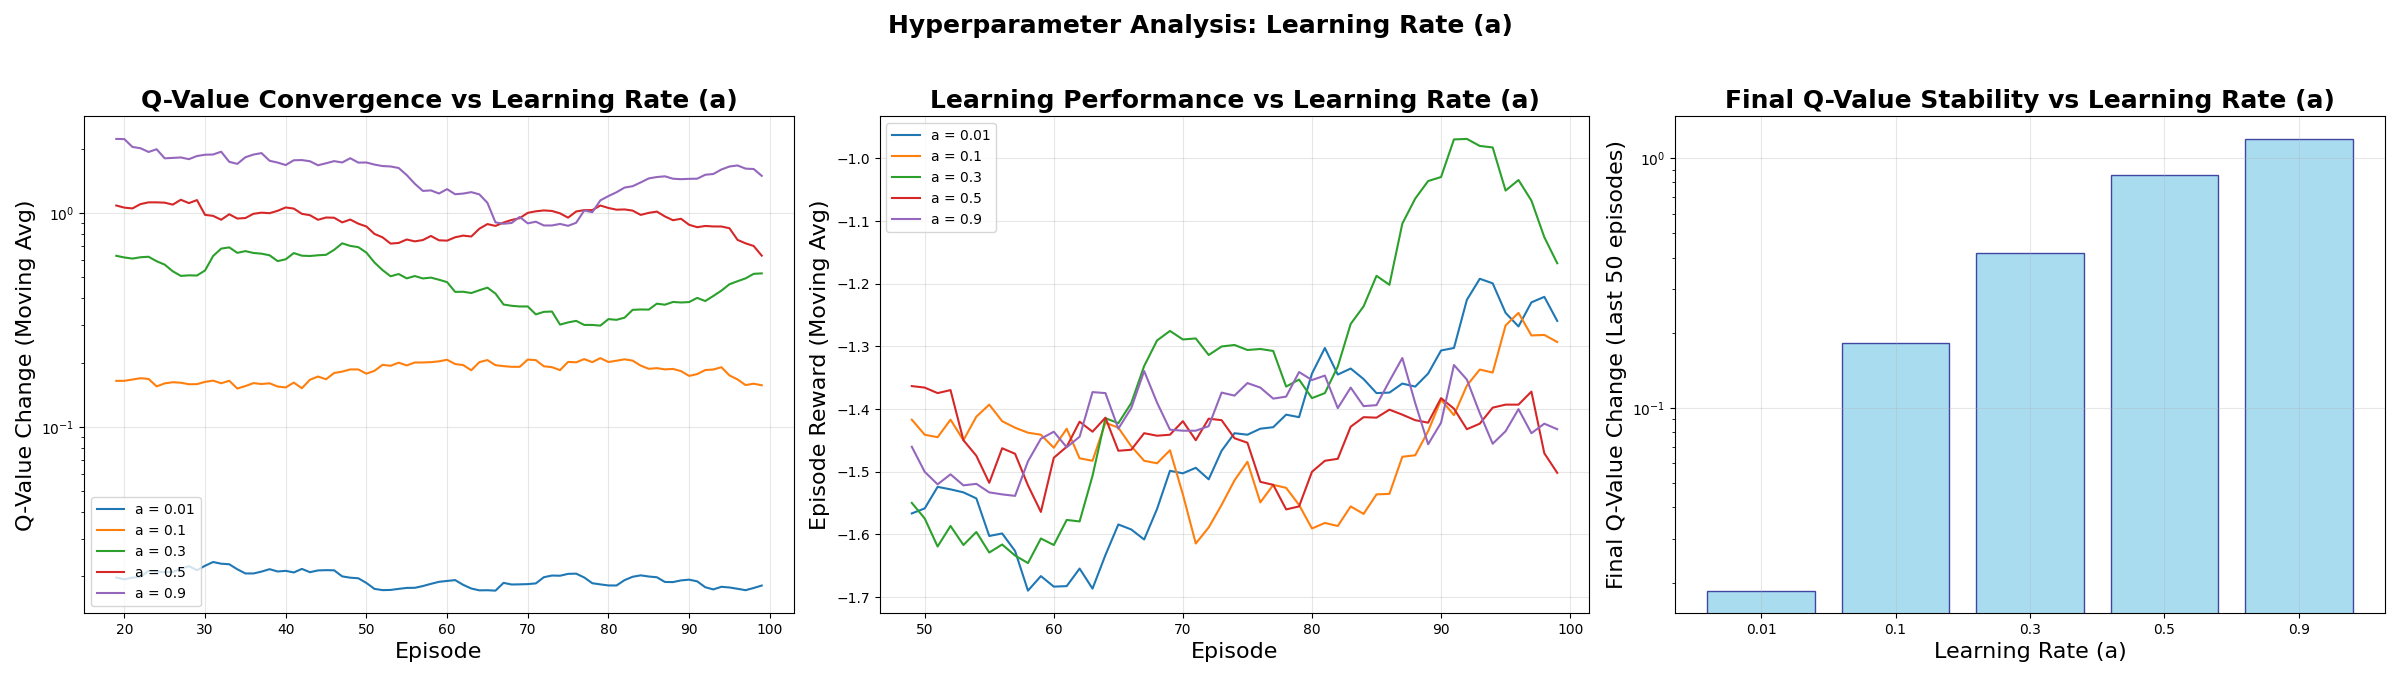
\includegraphics[width=\textwidth]{images/hyperparameter_analysis_alpha.png}
    \caption{Learning rate ($\alpha$) analysis showing that moderate values (0.1-0.3) achieve optimal balance between convergence speed and stability. High values cause instability while low values learn too slowly.}\label{fig:hyperparameter_alpha}
\end{figure}

\begin{figure}[H]
    \centering
    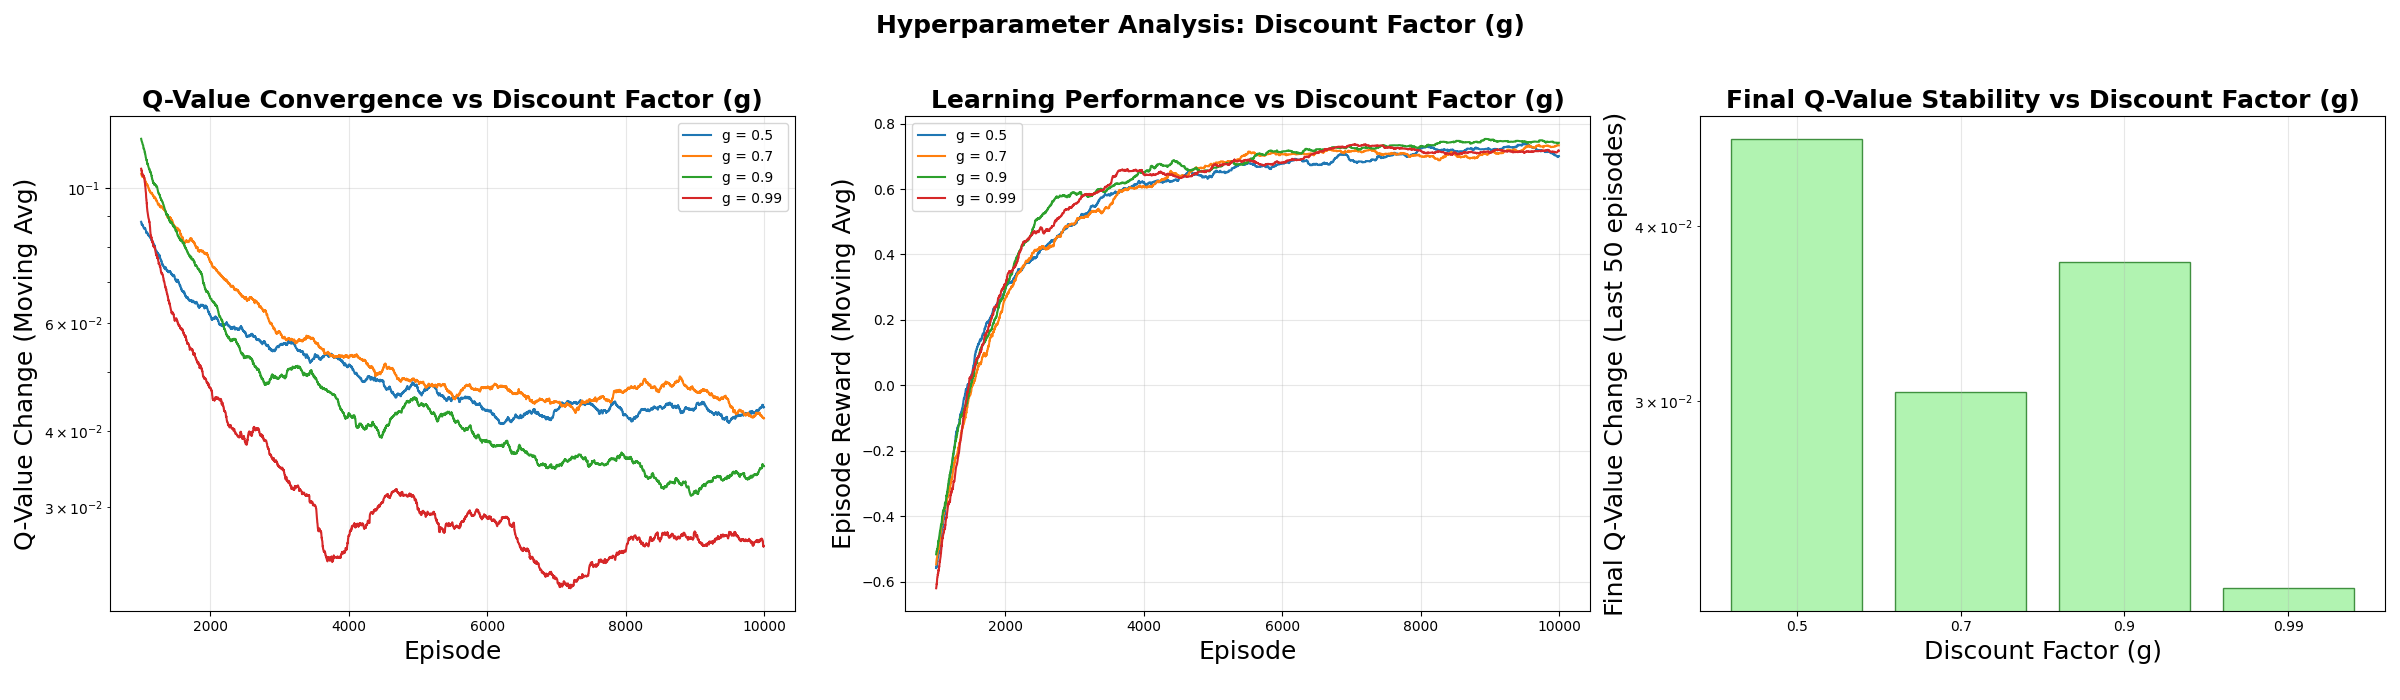
\includegraphics[width=\textwidth]{images/hyperparameter_analysis_gamma.png}
    \caption{Discount factor ($\gamma$) analysis showing that high values ($\gamma \geq 0.9$) are essential for optimal performance. Low values cause myopic behavior that prioritizes immediate rewards over the distant goal.}\label{fig:hyperparameter_gamma}
\end{figure}

\begin{figure}[H]
    \centering
    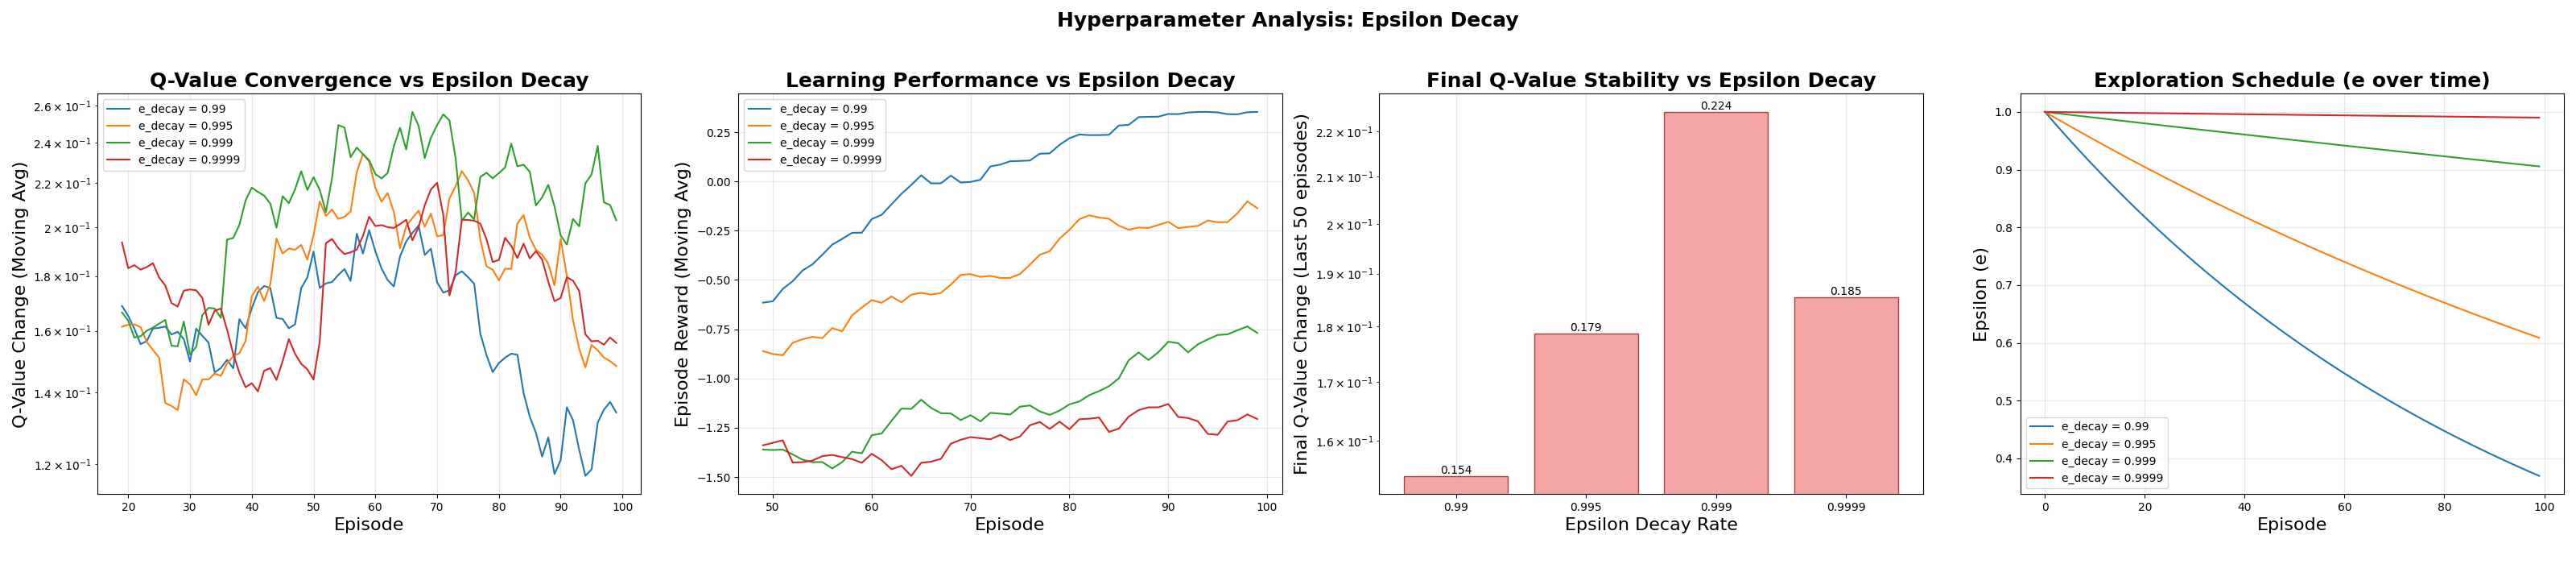
\includegraphics[width=\textwidth]{images/hyperparameter_analysis_epsilon_decay.png}
    \caption{Exploration schedule ($\epsilon$ decay) analysis revealing that moderate decay rates (0.999) optimally balance exploration and exploitation. Fast decay leads to premature convergence, slow decay wastes episodes on random actions.}\label{fig:hyperparameter_epsilon}
\end{figure}

\begin{figure}[H]
    \centering
    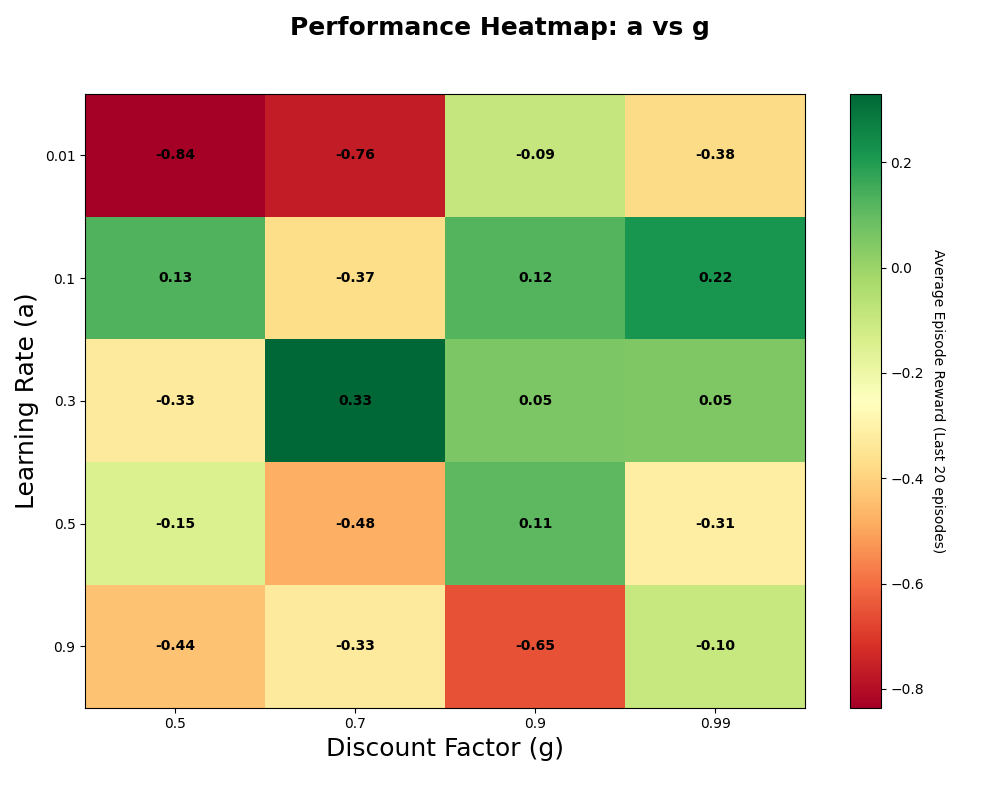
\includegraphics[width=0.7\textwidth]{images/hyperparameter_heatmap.png}
    \caption{Performance heatmap showing optimal combinations require high $\gamma$ (long-term planning) and moderate $\alpha$ (stable learning). The sharp performance drop at low $\gamma$ demonstrates its critical importance.}\label{fig:hyperparameter_heatmap}
\end{figure}

\begin{figure}[H]
    \centering
    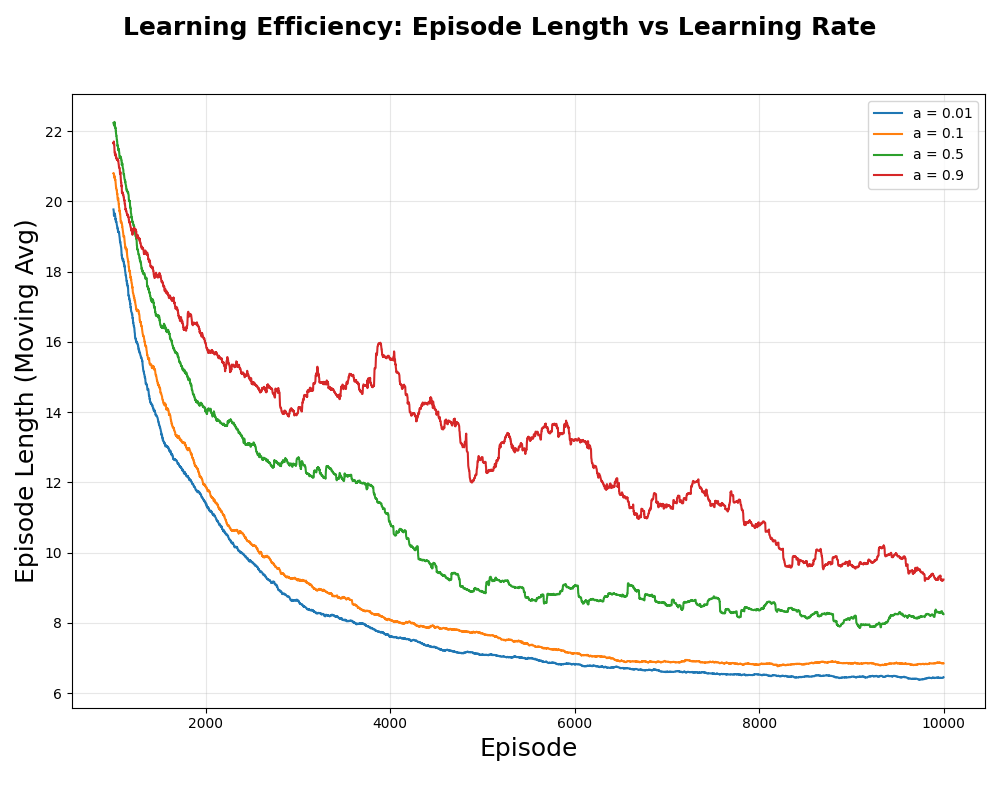
\includegraphics[width=0.7\textwidth]{images/hyperparameter_efficiency.png}
    \caption{Learning efficiency showing episode length evolution. Higher learning rates achieve rapid initial improvement but remain volatile, while moderate rates provide steady convergence to optimal path lengths.}\label{fig:hyperparameter_efficiency}
\end{figure}

\subsection{Understanding Convergence: Policy vs. Q-Values}
An important observation is that the agent's \textbf{policy converges much earlier than its Q-values}. The policy—what the agent decides to do—only depends on which action has the highest Q-value in a state. This relative ordering can stabilize long before the Q-values themselves stop changing numerically.

As shown in Figure~\ref{fig:convergence}, the number of policy changes (left panel) drops to zero after approximately 40 episodes, indicating the agent has discovered and committed to its final strategy. However, the total change in Q-values (right panel) continues to fluctuate throughout the entire training period. This occurs because the agent continues to refine its value estimates based on stochastic outcomes, even though the relative rankings that determine action selection have stabilized. This phenomenon demonstrates that effective decision-making can emerge well before complete value convergence, making Q-learning practical even with finite training time.

\begin{figure}[H]
    \centering
    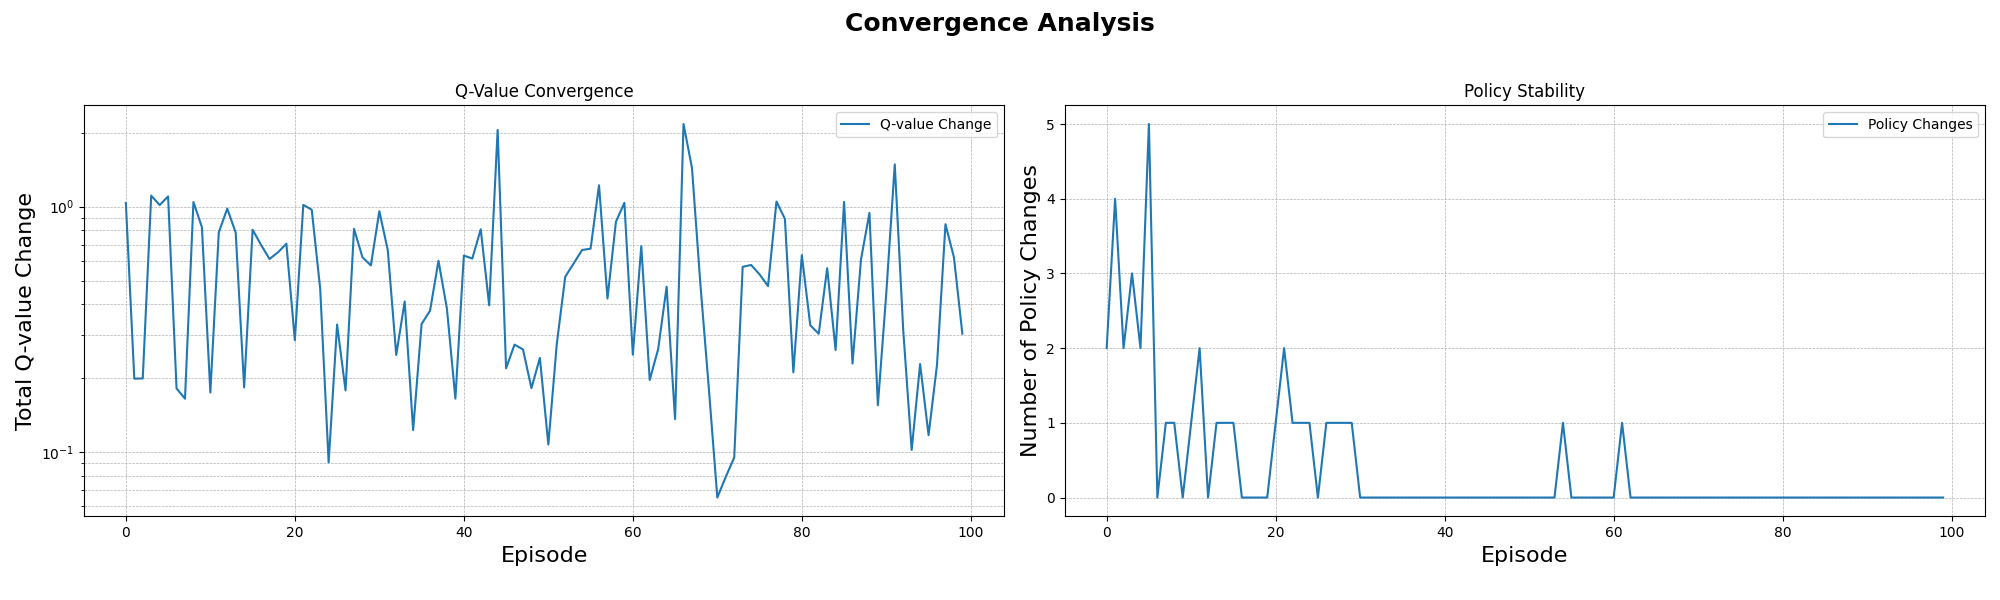
\includegraphics[width=0.8\textwidth]{images/convergence.png}
    \caption{Convergence analysis showing that policy stabilizes around episode 40 while Q-values continue fluctuating. This demonstrates that optimal decision-making emerges before complete value convergence.}\label{fig:convergence}
\end{figure}

\subsection{Comparing Standard vs. High-Risk Scenarios}
To see how the agent adapts to risk, we compared the learned policies from two different experiments: a standard run with a small penalty of -1, and a high-risk run with a massive penalty of -200.

\subsubsection{Case 1: Standard Penalty (-1)}
In the standard case, the agent learns an efficient and safe policy, shown in Figure~\ref{fig:policy_standard}. The optimal path is to move up the left side and across the top, safely avoiding the column with the penalty. This is a logical and effective strategy.

\begin{figure}[H]
    \centering
    \begin{tabular}{|c|c|c|c|}
        \hline
        $\rightarrow$ & $\rightarrow$ & $\rightarrow$ & \textbf{+1.0} \\
        \hline
        $\uparrow$ & WALL & $\uparrow$ & \textbf{-1.0} \\
        \hline
        $\uparrow$ & $\leftarrow$ & $\uparrow$ & $\leftarrow$ \\
        \hline
    \end{tabular}
    \caption{The agent's learned strategy for the standard problem (penalty = -1).}\label{fig:policy_standard}
\end{figure}

\subsubsection{Case 2: High-Risk Penalty (-200)}
When the penalty is increased to -200, the agent becomes extremely \textbf{risk-averse}, as seen in Figure~\ref{fig:policy_high_risk}. The new policy shows two key changes:
\begin{enumerate}
    \item \textbf{Strong Aversion:} Any state near the `-200` trap now has a policy that points sharply away from it. The policy in state (3,2), for example, changes from `$\uparrow$` to `$\leftarrow$`.
    
    \item \textbf{``Hunker Down'' Strategy:} In the bottom-right corner (4,1), the agent's policy is to move `$\downarrow$`, causing it to stay put. It has learned that doing nothing is safer than risking a move that might stochastically slip toward danger.
\end{enumerate}

This comparison makes it clear that the agent doesn't just learn a single path; it learns the true value of its actions and adapts its strategy to become more cautious as the environment becomes more dangerous.

\begin{figure}[H]
    \centering
    \begin{tabular}{|c|c|c|c|}
        \hline
        $\rightarrow$ & $\rightarrow$ & $\rightarrow$ & \textbf{+1.0} \\
        \hline
        $\uparrow$ & WALL & $\leftarrow$ & \textbf{-200.0} \\
        \hline
        $\uparrow$ & $\leftarrow$ & $\leftarrow$ & $\downarrow$ \\
        \hline
    \end{tabular}
    \caption{The agent's highly cautious strategy with a -200 penalty.}\label{fig:policy_high_risk}
\end{figure}

\subsection{Understanding the Q-Table: The Agent's Internal Knowledge}
To truly understand how the agent makes decisions, we can examine its internal ``cheat sheet''—the Q-table. This table contains the learned values for every action in every state, representing the agent's accumulated knowledge about the expected future rewards from each possible move.

Figure~\ref{fig:q_table_heatmap} shows the Q-values learned by the agent in the high-risk scenario (penalty = -200). Each subplot represents the Q-values for a specific action (North, South, East, West), with colors indicating the desirability of that action from each position:

\begin{itemize}
    \item \textbf{Red colors} indicate high Q-values (good actions)
    \item \textbf{Blue colors} indicate low Q-values (actions to avoid)
    \item The numerical values show the exact learned Q-values
\end{itemize}

Key observations from the Q-table visualization:
\begin{enumerate}
    \item \textbf{Goal attraction:} States near the goal (4,3) show high Q-values for actions that move toward it.
    \item \textbf{Penalty avoidance:} States near the penalty trap (4,2) show strongly negative Q-values for actions that might lead there, especially considering the stochastic movement.
    \item \textbf{Risk propagation:} The negative values ``spread'' from the penalty state to nearby states, showing how the agent learned to avoid not just the trap itself, but also risky positions nearby.
    \item \textbf{Safe path preference:} The left side of the grid shows consistently higher Q-values, reflecting the agent's learned preference for the safer route.
\end{enumerate}

This Q-table represents the culmination of 10,000 episodes of learning—a compact summary of everything the agent discovered about navigating this risky world.

\begin{figure}[H]
    \centering
    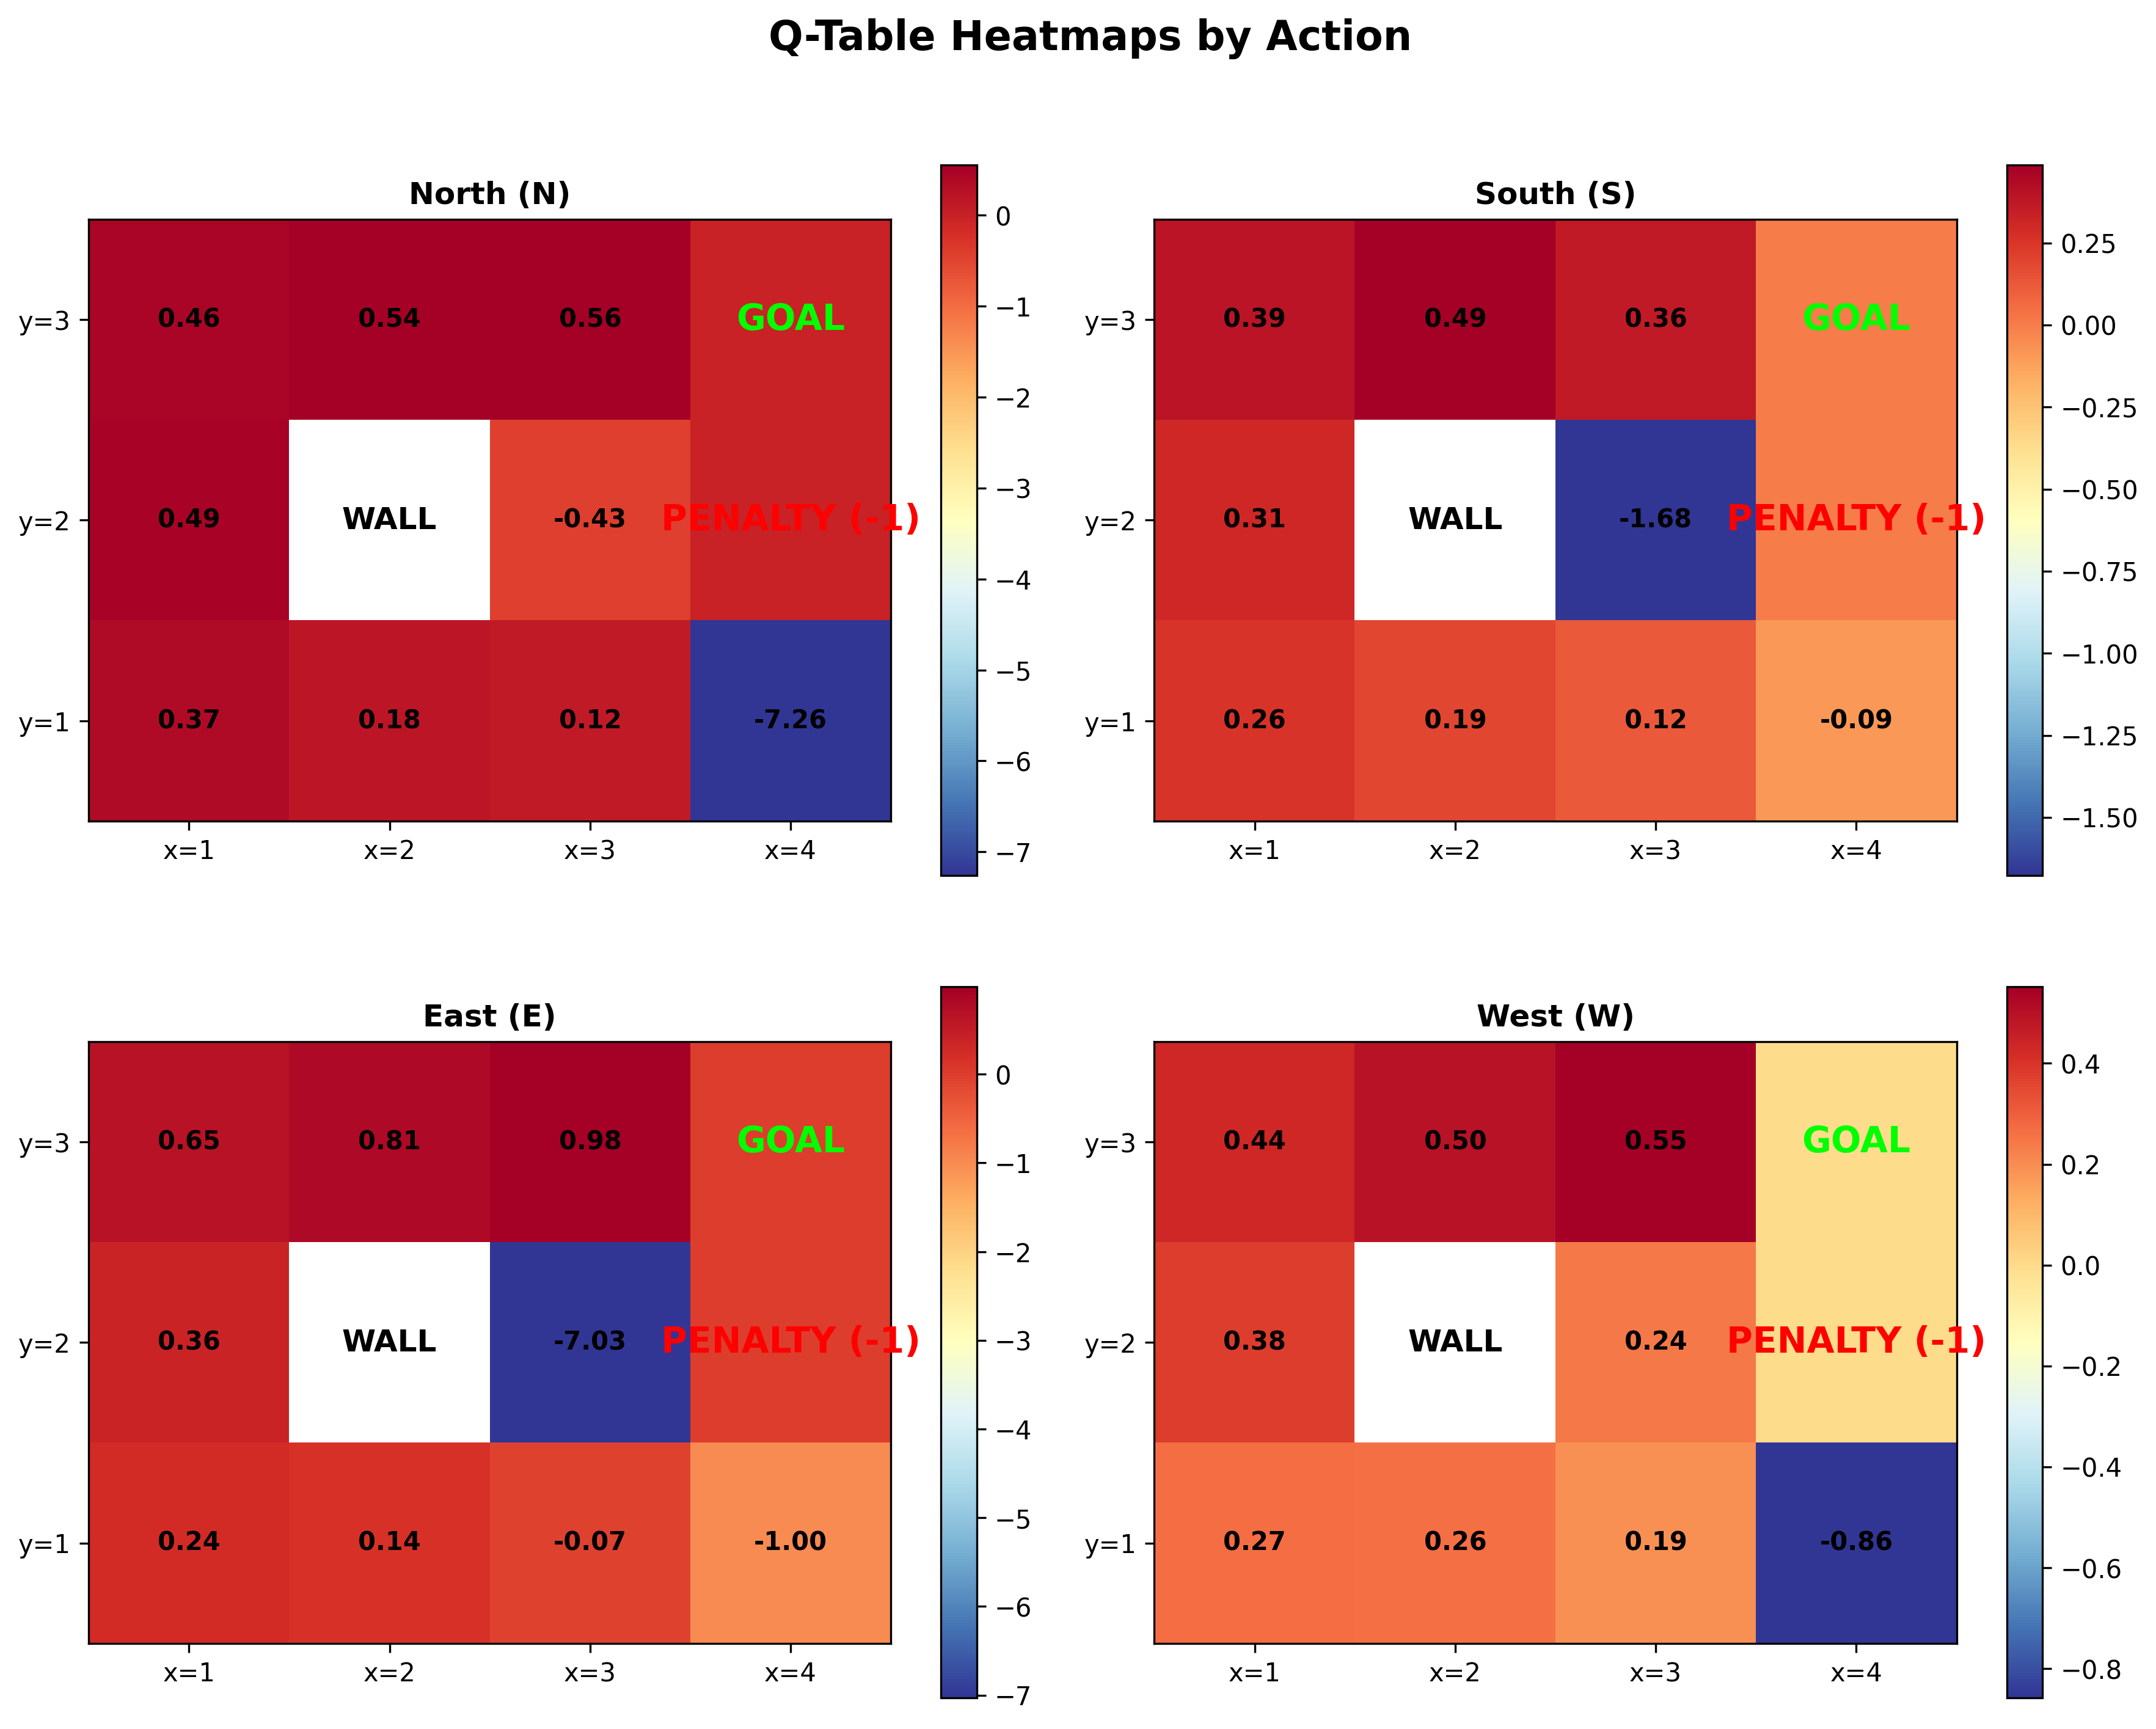
\includegraphics[width=\textwidth]{images/q_table_heatmap.png}
    \caption{Q-table heatmap showing learned Q-values for each action from every state. The visualization reveals how the agent learned to value actions based on their expected future rewards, with clear patterns of goal attraction and penalty avoidance.}\label{fig:q_table_heatmap}
\end{figure}

%===============================================================================
\section{Final Thoughts}
%===============================================================================
This experiment was a wonderful success. Our agent started with zero knowledge of its world and, through nothing but trial, error, and a simple reward mechanism, it developed sophisticated strategies. It proved that a simple learning algorithm can lead to surprisingly intelligent behavior, allowing an agent to adapt its level of risk aversion in response to the dangers of its environment. The complete code for this simulation is available on my \href{https://github.com/Jeevan-HM/RL-in-Robotics.git}{GitHub}.

\end{document}